\section{Laboratorium nr 3}

Podczas dzisiejszych zajęć omówiony zostanie temat projektowania filtrów zarówno tych o skończonej odpowiedzi impulsowej (ang. Finite Impulse Response, FIR) jak i~o~nieskończonej odpowiedzi impulsowej (ang. Infinite Impulse Response, IIR). Różnią się one złożonością obliczeniową, filtry nierekursywne są pod tym względem bardziej skomplikowane. Konieczna jest większą liczba współczynników filtra, aby osiągnąć strome zbocze w~paśmie przejściowym. Bardzo dużą natomiast zaletą filtrów typu FIR jest fakt, że są one zawsze stabilne. Nie ma takich wartości wagowych filtra, które spowodują że sygnał wyjściowy się wzbudzi i~wzrośnie do nieskończoności. Dodatkową zaletą filtrów o skończonej odpowiedzi impulsowej jest liniową charakterystyka fazowo-częstotliwościowa co jest szczególnie pożądane przy niektórych typach sygnałów np. w aparaturze medycznej. 

\subsection{Odpowiedzi częstotliwościowe filtrów cyfrowych}
Filtry (niezależnie od typu) mogą być opisane przez tzw. charakterystyki częstotliwościowe. Opisują one jak dany filtr ,,działa'' na sygnał wejściowy. Filtr może odpowiednio wzmacniań/tłumić dane pasma częstotliwości oraz dodatkowo może dane częstotliwości przesuwać w fazie. Na rysunku nr~\ref{lab3/fig/frequenciesResponses} zostały pokazane odpowiedzi częstotliwościowe dwóch filtrów: dolnoprzepustowego FIR (lewa kolumna) oraz wszystkoprzepustowego filtra IIR (prawa kolumna).
\begin{figure}[hbt!]
	\centering
	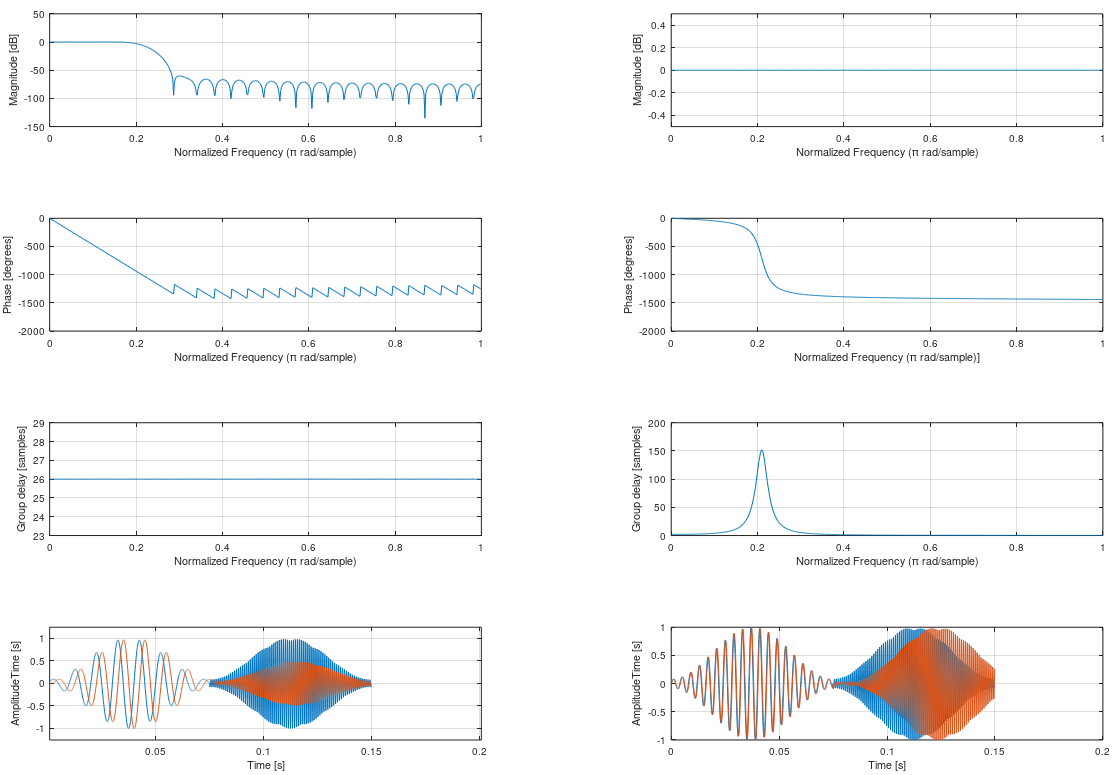
\includegraphics[width=0.95\linewidth]{images/frequenciesResponses.png}
	\caption{Odpowiedzi częstotliwościowe, opóźnienie grupowe oraz przykład filtracji przykładowego dolnoprzepustowego filtra FIR (lewa kolumna) oraz wszystkoprzepustowego IIR (prawa kolumna).}
	\label{lab3/fig/frequenciesResponses}
\end{figure}
Na wykresach w pierwszym wierszu można zaobserwować jak pokazane filtry będą zmieniały amplitudy sygnałów wejściowych w zależności od częstotliwości. Pierwszy z~nich będzie ,,przepuszczał'' częstotliwości od $0$ do $0.2$ unormowanej względem jedynki częstotliwości Nyquista. Inaczej mówiąc, przy założeniu, że częstotliwość próbkowania $F_s$ wynosi $10000~Hz$ (częstotliwość Nyquista $\frac{F_s}{2} = 5000~Hz)$ do filtr przedstawiony w~lewej kolumnie będzie przenosił częstotliwości od $0$ do $1000~Hz$ ($5000\cdot0.2$). Natomiast filtr przedstawiony w~prawej kolumnie, ponieważ wzmocnienie wynosi $0~dB$ dla całego pasma, nie będzie tłumił/wzmacniał żadnej częstotliwości, kolokwialnie mówiąc ,,przepuści wszystko''.

W drugim wierszu natomiast zostały pokazane charakterystyki fazowe filtrów. Po lewej stronie można zaobserwować liniowy wykres (z wyjątkiem skoków o wartość równą $\pi$ w miejscach, gdzie charakterystyka amplitudowa zmienia znak). Wszystko przepuszczający filtr natomiast ma nieliniową charakterystykę fazową (co jest typowe dla filtrów rekursywnych IIR). Aby dowiedzieć się o jaką wartość dane częstotliwości w sygnale zostaną przesunięte należy policzyć pochodną z charakterystyki fazowej~\ref{lab3/eq/groupDelay}. Wykresy tych pochodnych (tzw. przesunięcia grupowe) zostały pokazane w trzecim wierszu. 
\begin{equation}\label{lab3/eq/groupDelay}
	\tau_g = - \frac{d \phi}{d \omega}
\end{equation}

W ostatnim wierszu zaprezentowano efekt działania filtrów na sygnał wejściowy składający się z dwóch funkcji typu sinus o częstotliwościach odpowiednio $100$ i $1100~Hz$ występujących jeden po drugim. Inaczej mówiąc wektor wejściowy składa się najpierw z jednej funkcji sinus w przedziale od zera do połowy wektora wejściowego, potem następuje druga funkcja sinus o większej częstotliwości. Na wykresie w~dolnym lewym rogu można - z łatwościom - zaobserwować, że pierwsza połowa wektora wejściowe (o częstotliwości $100~Hz$) nie została stłumiona, w przeciwieństwie do drugiej której amplituda uległa zmniejszeniu. Jednocześnie warto zauważyć, że wszystkie częstotliwości zostały przesunięte w czasie o taką samą liczbę próbek, z~wykresu opóźnienia grupowego można odczytać, że tą wartością jest $26$ próbek. 

Nieco inaczej wygląda sytuacja na wykresie znajdującym się w dolnym prawym rogu (filtr wszystkoprzepuszczający). Żadna z częstotliwości nie uległa stłumieniu, nie powinno to dziwić zważywszy na fakt, że charakterystyka amplitudowa wynosi $0~dB$ w całym paśmie. Natomiast wartym zauważenia jest fakt, iż filtr ten przesuwa z fazie jedynie częstotliwości około $1100~Hz$ ($0.22$ częstotliwości Nyquista). Widać to wyraźnie na wykresie, gdzie część o niższej częstotliwości niemal w ogóle nie uległa przesunięciu, natomiast częstotliwość $1100~Hz$ jest wyraźnie przesunięta w fazie o około $150$ próbek.

Aby narysować charakterystyki częstotliwościowe filtrów (zarówno FIR jak i IIR) w programie MATLAB/Octave można użyć funkcji \texttt{freqz(b,a)}. W~najprostszym przypadku przyjmuje ona dwa wektory będące współczynnikami filtra, odpowiednio \texttt{b} to współczynniki licznika filtra, natomiast \texttt{a} to współczynniki mianownika filtra (w przypadku filtrów FIR, gdzie mianownik równa się jedności należy przekazać liczbę \texttt{1}). Na rysunku~\ref{lab3/fig/freqzFunction} pokazano charakterystyki częstotliwościowe filtra typu FIR o unormowanej częstotliwości granicznej $0.3$ i rzędzie równym $51$. Zakładając, że \texttt{b} to wektor współczynników licznika filtra, to pokazany wykres otrzymano wywołując funkcję \texttt{freqz(b,1)}.

\begin{figure}[hbt!]
	\centering
	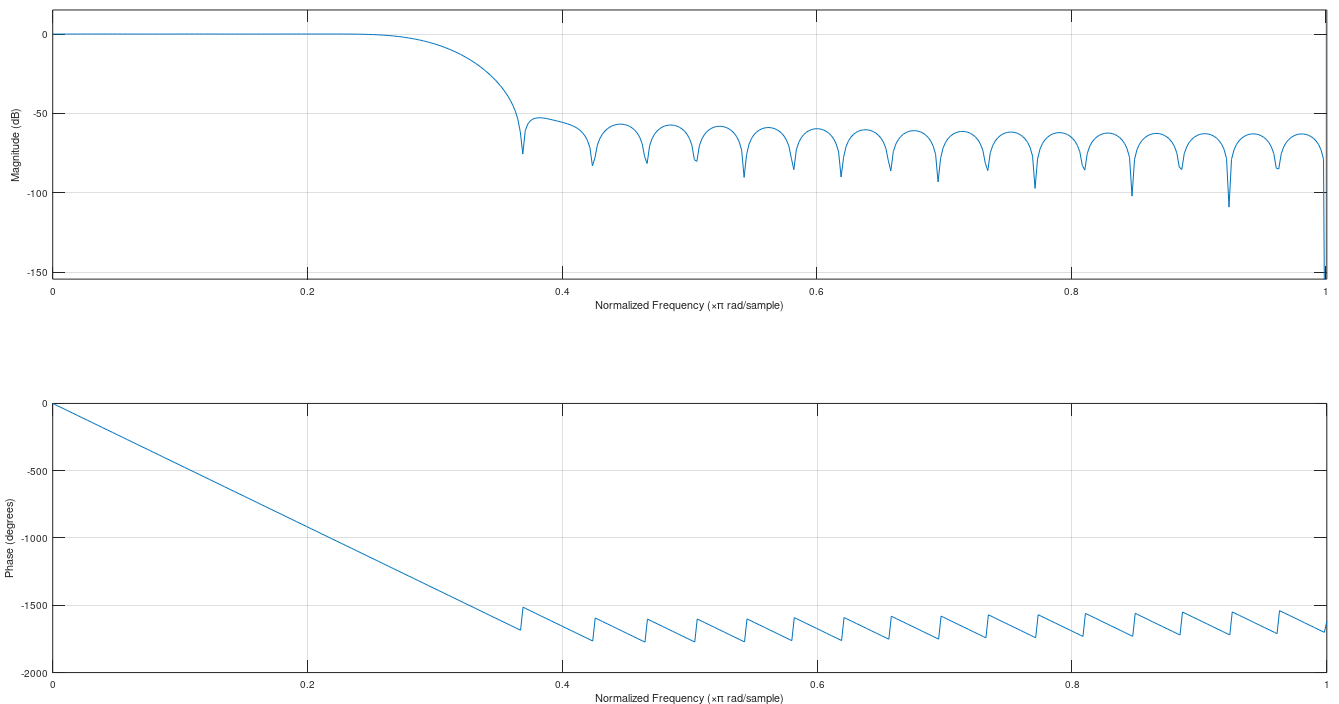
\includegraphics[width=0.9\linewidth]{images/freqzFunction.png}
	\caption{Charakterystyki częstotliwościowe dla filtru typu FIR o unormowanej częstotliwości granicznej $0.3$ i rzędzie równym $51$}
	\label{lab3/fig/freqzFunction}
\end{figure}

\subsection{Filtry o skończonej odpowiedzi impulsowej (FIR)}
Filtry nierekursywne FIR nie posiadają sprzężenie zwrotnego. Każda próbka wyjściowa jest sumą ważoną próbek z~poprzednich chwil czasu~\ref{lab3/eq/firFilterEquation}. Na rysunku nr~\ref{lab3/fig/firFilterDirectForm} pokazano schemat blokowy filtra typu FIR. Zaznaczone na nim kwadraty z $z^{-1}$ oznaczają opóźnienie próbki o wartość jeden w dziedzinie operatora $Z$.

\begin{equation}\label{lab3/eq/firFilterEquation}
	y[n] = b_0 x[n] + b_1 x[n-1] + ... + b_N[x-N] = \sum_{i=0}^{N}b_i\cdot x[n-i]
\end{equation}

\begin{figure}[hbt!]
	\centering
	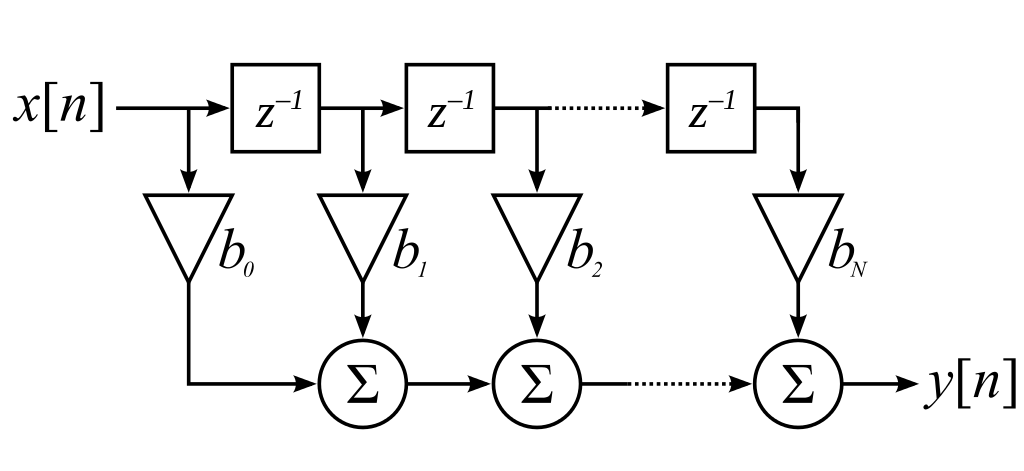
\includegraphics[width=0.7\linewidth]{images/firFilterDirectForm.png}
	\caption{Bezpośrednia forma dyskretnoczasowego filtru FIR rzędu $N+1$.}
	\label{lab3/fig/firFilterDirectForm}
\end{figure}

Filtry FIR można projektować na wiele analitycznych sposobów. Projektowanie filtrów sprawdza się do wyznaczenia wartości współczynników wagowych $b_0, b_1, ... b_N$. Jedną z~prostszych metod, z której korzysta funkcja \texttt{fir1} programu MATLAB/Octave jest metoda okien. Jest ona stosunkowo prosta pod względem zarówno teoretycznym jak i~implementacyjnym. Analitycznie wzory na różne rodzaje filtrów FIR wyprowadza się z odpowiedzi impulsowej ,,idealnego'' filtru dolnoprzepustowego. Pozostałe filtry mogą być obliczone jako superpozycja filtrów dolnoprzepustowych o różnych częstotliwościach granicznych oraz filtra ,,wszechprzepustowego''~\footnote{Filtr ,,wszechprzepustowy'' posiada charakterystykę amplitudową, która jest równa jedności w~całym paśmie. Może posłużyć do modyfikacji fazy sygnału bez wpływu na jego amplitudę. Jego odpowiedź impulsowa jest deltą Kroneckera $H(e^{j\Omega}) = 1$.}. Na tych zajęciach nie zgłębiając teoretycznych aspektów projektowania filtrów typu FIR, wykorzystana zostanie wspomniana funkcja \texttt{fir1()} programu MATLAB/Octave. Pozwala ona na wyznaczenie współczynników filtra wcześniej wspomnianą metodą okien. 


Poniżej został pokazany listing~\ref{lab3/lst/chirpFilterOut} ukazujący filtrację sygnału świergotowego\footnote{Sygnał świergotowy jest sygnałem, w którym częstotliwość zmienia się (rośnie albo maleje) liniowo w~czasie}. Ten rodzaj modulowanego sygnału idealnie nadaje się do pokazania idei samej filtracji. Częstotliwość zmienia się w nim liniowo i po jego wymnożeniu z odpowiedzią impulsową filtra cześć sygnału powyżej pewnej częstotliwości zostanie wytłumiona. Do stworzenia takiego sygnału można wykorzystać funkcję \texttt{chirp(t, f0, t1,f1)}, gdzie \texttt{t} jest wektorem czasu, \texttt{f0} częstotliwością początkową w chwili $t=0$, \texttt{t1} chwilą czasu, w której sygnał osiąga częstotliwość \texttt{f1}. Do wyznaczenia współczynników filtra typu FIR wykorzystano funkcję \texttt{fir1(n, wn)}. Przyjmuje ona minimum dwa argumenty, pierwszym (\texttt{n}) jest rząd filtra, drugim natomiast unormowana względem częstotliwości Nyquista częstotliwość odcięcia. W poniższym przykładzie częstotliwość próbkowania $F_s$ została ustawiona na $12000~Hz$, częstotliwość Nyquista w~tym przypadku wynosi połowę $F_s$ t.j. $F_n=\frac{F_s}{2} = 6000~Hz$. Chcąc otrzymać współczynniki filtru, który odfiltruje częstotliwości sygnału większe niż $1500~Hz$, należy jako argument \texttt{wn} przekazać liczbę $0.25$, ponieważ $6000\cdot0.25 = 1500~Hz$.


Aby wymnożyć sygnał filtrowany ze współczynnikami filtra, najlepiej użyć funkcji \texttt{filter(b,a,y)}, gdzie \texttt{b} to kolejne wagi licznika filtra, \texttt{a} to kolejne wagi mianownika filtra, \texttt{y} filtrowany wektor próbek. W~poniższym przypadku drugi argument wyniósł \texttt{1} ponieważ filtr typu FIR nie posiada mianownika, współczynników rekursywnych. W przypadku systemów FIR możliwe jest również wykorzystanie funkcji liczącej splot~\texttt{conv(a,b)} \ref{lab1/sec/convolution} \footnote{Funkcja \texttt{filter} jest odpowiednią funkcją zarówno dla filtrów FIR jak i IIR. Funkcja licząca splot \texttt{conv} pobiera dwa wejścia i zwraca ich splot, dlatego w~tym przypadku \texttt{conv(x,y)} i \texttt{filter(h,1,x)} zwrócą ten sam wynik. Jedynka w filtrze mówi nam o tym, że współczynnik rekursywny filtru wynosi jeden. Jeśli jednak mamy do czynienia z filtrem IIR to nie możemy wykorzystać \texttt{conv}.}.




\begin{lstlisting}[caption=Filtracja sygnału świergotowego zmieniającego liniowo częstotliwość w przedziale od $0$ do $3~kHz$ , label=lab3/lst/chirpFilterOut]
	Fs = 12000;             % Sampling frequency
	t = 0:1/Fs:1;           % Time vector
	y = chirp(t,0,1,3000);  % Generate samples of linear swept-frequency cosing signal. 0 frequency at t=0 to 3 kHz at t=1
	
	subplot(2,1,1);
	plot(t,y);
	title('Input chirp signal with frequency changing from 0 to 3 kHz');
	xlabel('Time [s]')
	ylabel('Amplitude');
	
	n = 100;
	wn = 0.25;                % Nyquist frequency Fs/2 = 6000. Cut off frequency: 6000*0.25 = 1500 Hz
	b = fir1(n, wn);          % Create  n order lowpass filter coefficient
	yFiltered = filter(b,1,y);%Use filter function to filterout y signal
	subplot(2,1,2);
	plot(t,yFiltered);
	title('Chirp signal with filter out frequency above 1.5 kHz');
	xlabel('Time [s]')
	ylabel('Amplitude');
\end{lstlisting}

\begin{figure}[hbt!]
	\centering
	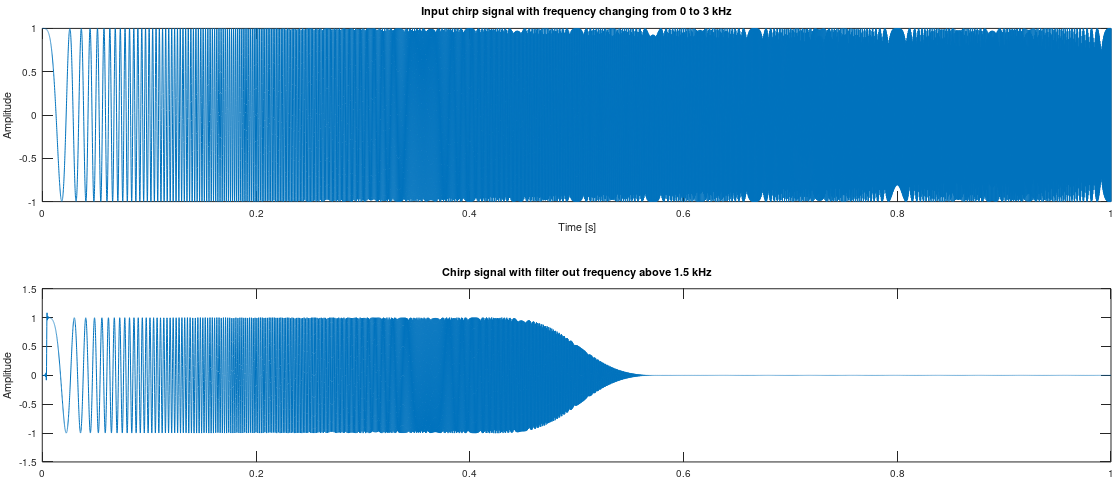
\includegraphics[width=0.9\linewidth]{images/chirpFilterOut.png}
	\caption{Filtracja sygnału świergotowego, zmieniającego liniowo częstotliwość w przedziale od $0$ do $3~kHz$}
	\label{lab3/fig/chirpFilterOut}
\end{figure}


Na listingu~\ref{lab3/lst/firFiltersExample} pokazano sposób projektowania filtrów nierekursywnych (FIR) odpowiednio dolnoprzepustowego, górnoprzepustowego oraz środkowoprzepustowego. W pierwszej kolejności utworzono sygnał składający się z trzech funkcji kosinus o częstotliwościach odpowiednio $50,~500,~1000~[Hz]$, częstotliwość próbkowania w tym przykładzie została ustawiona na $5000~Hz$. Sygnał poddawany filtracji pokazano na rysunku~\ref{lab3/fig/firFiltersExample}. W~pierwszym wierszu po lewej stronie sygnał został pokazany w~dziedzinie czasu, po prawej natomiast w~dziedzinie częstotliwości po wykonaniu dyskretnego przekształcenia Fouriera za pomocą funkcji \texttt{fft} - uwaga funkcja \texttt{plotFFT} nie jest domyślną funkcją programu MATLAB/Octave, jest to funkcja napisana podczas drugich laboratoriów~\ref{lab2/lst/fftExample}).

Następnie z wykorzystaniem funkcji \texttt{fir1(n, Wn)} obliczono współczynniki filtrów odpowiednio dolnoprzepustowego (tłumione są częstotliwości przekraczające $0.1\cdot f_N = 250~Hz$). Dalej obliczono współczynniki filtra górnoprzepustowego (tłumione są częstotliwości poniżej $0.3\cdot f_N = 750~Hz$). Warto zwrócić uwagę na przekazanie do funkcji \texttt{fir1} dodatkowego trzeciego argumentu \texttt{'high'}, który mówi, że chcemy obliczyć współczynniki filtra górnoprzepustowego (domyślnie przyjmowany jest argument \texttt{'low' }). Na koniec pokazano filtr środkowoprzepustowy w przypadku którego konieczne jest przekazanie wektora zawierającego przedział częstotliwości, które będą ,,przepuszczane'' przez filtr w tym przypadku \texttt{[0.1 0.3]} (stłumiona zostaną wszystkie częstotliwości poza przedziałem $f \in [250,~750]~Hz$).




\begin{lstlisting}[caption=Filtracja sygnału poszczególnych składowych z sygnały $y(t)$ , label=lab3/lst/firFiltersExample]
	Fs = 5000;            % Sampling frequency
	T = 1/Fs;             % Sampling period       
	L = 5000;             % Signal length
	t = (0:L-1)*T;        % Time vector
	y = 1.0*cos(2*pi*50*t) + 0.5*cos(2*pi*500*t) + 2*cos(2*pi*1000*t); % Prepare signal
	subplot(4,2,1); plot(t, y); 
	title('Input signal');xlabel('Time [s]'); 
	ylabel('Amplitude'); axis([0.1 0.15]);
	
	% Fourier transform of y
	subplot(4,2,2); plotFFT(y, Fs);
	
	
	% Filter out higher frequency
	n = 51;
	Wn = 0.1;
	b = fir1(n,Wn);
	yLP = filter(b,1,y);
	subplot(4,2,3); plot(t, yLP);
	title('Input signal after low pass filter');xlabel('Time [s]'); 
	ylabel('Amplitude'); axis([0.1 0.15]);
	subplot(4,2,4); plotFFT(yLP, Fs);
	
	% Filter out lower frequency
	n = 51;
	Wn = 0.3;
	b = fir1(n,Wn, 'high');
	yHP = filter(b,1,y);
	subplot(4,2,5); plot(t, yHP);
	title('Input signal after high pass filter');xlabel('Time [s]'); 
	ylabel('Amplitude'); axis([0.1 0.15]);
	subplot(4,2,6); plotFFT(yHP, Fs);
	
	% Filter out lower ang higher frequency (band pass filter)
	n = 51;
	Wn = [0.1 0.3];
	b = fir1(n,Wn);
	
	yBP = filter(b,1,y);
	subplot(4,2,7); plot(t, yBP); 
	title('Input signal after band pass filter');xlabel('Time [s]'); 
	ylabel('Amplitude'); axis([0.1 0.15]);
	subplot(4,2,8); plotFFT(yBP, Fs);
\end{lstlisting}
\begin{figure}[hbt!]
	\centering
	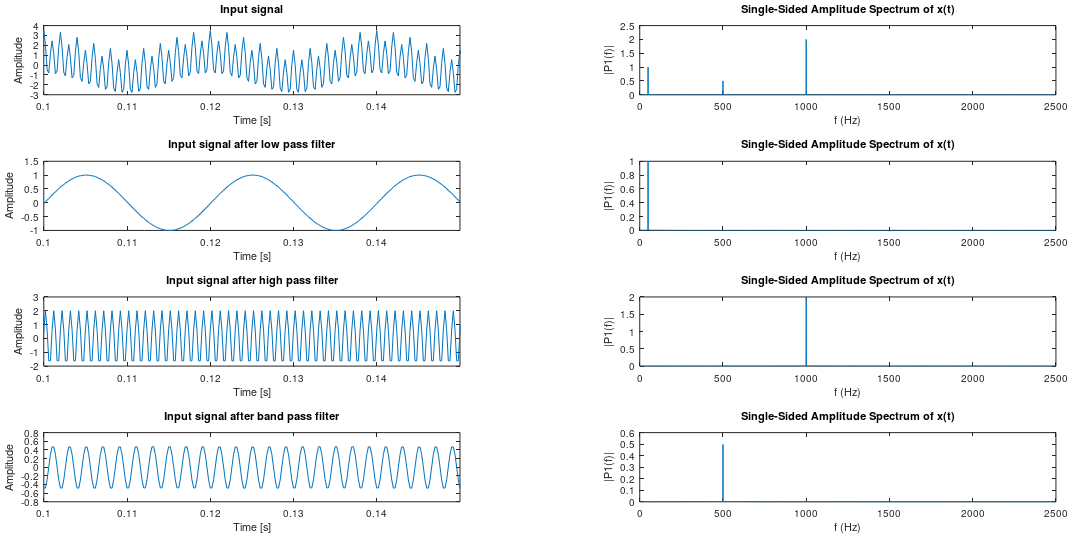
\includegraphics[width=0.95\linewidth]{images/firFiltersExample.png}
	\caption{Filtracja poszczególnych składowych sygnału $y(t)$}
	\label{lab3/fig/firFiltersExample}
\end{figure}




\subsection{Filtry o skończonej odpowiedzi impulsowej (IIR)}
Filtry typu IIR są systemami rekursywnymi tzn. do obliczenia wyjścia filtra wykorzystywane są próbki wejściowe (jak w filtrach FIR) oraz poprzednie próbki wyjściowe. Inaczej mówiąc filtry te posiadają sprzężenie zwrotne. Wzór na n-tą próbkę wyjściową filtru IIR został pokazany poniżej~\ref{lab3/eq/iirFilterEquation}.

\begin{equation}\label{lab3/eq/iirFilterEquation}
	y[n] = \frac{1}{a_0} (b_0 x[n] + b_1 x[n-1] + ... + b_P x[n-P] - a_1 y[n-1] - a_2 y[n-2] - ... - a_Q y[n-Q])
\end{equation}
,gdzie: $P$ jest rzędem wielomianu licznika, $Q$ jest rzędem wielomianu mianownika.

Do najważniejszych zalet filtrów IIR należy zaliczyć fakt, iż specyfikacje wymagane od filtra (np. stromość zbocza) udaje się osiągnąć układem o znacznie niższym rzędzie niż w przypadku układów nierekursywnych. Wśród wad należy nadmienić, że sprzężenie zwrotne przy złym zaprojektowaniu filtru może powodować utratę jego stabilności. Dodatkowo w przeciwieństwie do filtrów FIR nie posiadają one liniowej charakterystyki fazowej. Oznacza to, że takie filtry różnie przesuwają w fazie różne częstotliwości. W wielu układach warunek liniowej charakterystyki fazowej jest wymagany np. przy sygnałach związanych z urządzeniami medycznymi.

Klasyczne filtry IIR są projektowane z wykorzystaniem ich analogowych prototypów. W programie MATLAB/Octave typowe filtry analogowe takie jak filtr Butterwortha, Czebyszewa typu I, Czebyszewa typu II czy filtr eliptyczny za pomocą odpowiednich transformacji mogą być wykorzystane do wyznaczenia cyfrowych odpowiedników. Do obliczenia współczynników wspomnianych filtrów należy skorzystać z funkcji odpowiednio: \texttt{butter()}, \texttt{cheby1()}, \texttt{cheby2()}, \texttt{ellip()}. Proces obliczania współczynników filtrów jest analogiczny jak w przypadku filtrów FIR~\ref{lab3/lst/iirFiltersExamples}. 

\begin{lstlisting}[caption=Przykłady filtrów rekursywnych, label=lab3/lst/iirFiltersExamples]
[b,a] = butter(5,0.4);                    % Lowpass Butterworth
[b,a] = cheby1(4,1,[0.4 0.7]);            % Bandpass Chebyshev Type I
[b,a] = cheby2(6,60,0.8,'high');          % Highpass Chebyshev Type II
[b,a] = ellip(3,1,60,[0.4 0.7],'stop');   % Bandstop elliptic
\end{lstlisting}

Filtr Butterworth'a charakteryzuje się możliwe najbardziej płaską charakterystyką amplitudową w paśmie przenoszenia kosztem mniejszego niż inne filtry zbocza w paśmie przejściowym. Filtr Czebyszewa typu I posiada zafalowania w paśmie przepustowym oraz płaski przebieg w paśmie zaporowym. Natomiast filtry Czebyszewa typu II posiada płaską charakterystykę w paśmie przepustowym i zafalowania w paśmie zaporowym. W obu przypadkach (typ I oraz II) filtr posiada strome zbocze w paśmie przejściowym. Identyczne zafalowania z paśmie przepustowym i zaporowym ma natomiast filtr eliptyczny, który jednocześnie charakteryzuje się niemal pionowym zboczem w paśmie przejściowym.



\subsection{Zadania}
\subsubsection{Filtracja sygnału świergotowego}
Analogicznie jak zostało pokazane na listingu nr~\ref{lab3/lst/chirpFilterOut} utwórz sygnał świergotowy o~zmieniającej się liniowo częstotliwości w przedziale $f\in[0, 4000]~Hz$. Częstotliwość próbkowania $F_s$ możne zostać ustawiona na wartość $10000~Hz$.

Utwórz \textbf{filtr górnoprzepustowy}, który odfiltruje wszystkie częstotliwości w przedziale $f\in[0,1000]~Hz$. Aby uzyskać współczynniki filtra górnoprzepustowego wywołaj funkcję \texttt{fir1}, z dodatkowym trzecim argumentem \texttt{'high'}: \texttt{b = fir1(n, wn,'high')}. Wyniki przedstaw na współdzielonym wykresie, analogicznie jak zostało to pokazane na rysunku nr~\ref{lab3/lst/chirpFilterOut}.

\subsubsection{Filtracja poszczególnych składowych sygnału}
Podobnie jak na listingu~\ref{lab3/lst/firFiltersExample} utwórz sygnał składający się z trzech składowych o częstotliwościach odpowiednio $250,~750,~1500~Hz$ i dowolnych amplitudach. Do tego sygnału dodaj szum biały o~rozkładzie normalnym (\texttt{y= ... + randn(1,length(t))}). 

Następnie wykorzystując funkcję \texttt{fir1()} usuń z sygnału odpowiednio:
\begin{itemize}
	\item składową o częstotliwości $250~Hz$,
	\item składową o częstotliwości $1500~Hz$,
	\item składową o częstotliwości $750~Hz$ (stwórz filtr środkowozaporowy, analogicznie jak filtr środkowoprzepustowy pokazany na listingu~\ref{lab3/lst/firFiltersExample}, ale z dodanym trzecim argumentem \texttt{'stop'} np. \texttt{fir1(n, Wn, 'stop')}).
\end{itemize}

Wykresy umieść na współdzielonym wykresie analogicznie jak pokazano na rysunku~\ref{lab3/fig/firFiltersExample}. Zwróć uwagę, że szum biały został usunięty jedynie w~obszarach pasma zaporowego tzn. dla filtru dolnoprzepustowego jedynie od częstotliwości granicznej, leżącej gdzieś powyżej $250~Hz$, w zależności od zaprojektowanego filtru. Proszę mieć na uwadze, że szum biały składa się z częstotliwości znajdujących się w całym zakresie widma.



\subsubsection{Stromość pasma przejściowego, a długość filtra FIR}
Oblicz współczynniki trzech filtrów dolnoprzepustowych o częstotliwości granicznej \texttt{Wn=0.5} oraz o różnych rzędach np.: 
\begin{lstlisting}
b1 = fir1(5, 0.5);
b2 = fir1(25, 0.5);
b3 = fir1(50, 0.5);
\end{lstlisting}
Następnie narysuj po kolei charakterystyki częstotliwościowe tych filtrów za pomocą funkcji \texttt{freqz(b1,1), freqz(b2,1)} oraz \texttt{freqz(b3,1)}. Zwróć uwagę, że im wyższy rząd filtru tych bardziej wąskie pasmo przejściowe (pomiędzy pasmem przepustowym, a zaporowym). Warto również zauważyć, iż im wyższy rząd filtru tym bardziej strome nachylenie liniowej charakterystyki fazowej, co przekłada się na większe przesunięcie fazowe filtru o wyższym rzędzie. Aby narysować te charakterystyki na współdzielonym wykresie (\texttt{subplot}) można posłużyć się poniższym fragmentem kodu.
\begin{lstlisting}
[y,x] = freqz(b1,1);
subplot(311)
plot(x./pi, 10*log10(abs(y)));grid on; %x./pi because of normalization, 10*log10() because of logarithmic scale (in dB)
%...
\end{lstlisting}

\subsubsection{Sprawdzenie charakterystyk amplitudowych filtrów rekursywnych (IIR)}
Za pomocą funkcji programu MATLAB/Octave wyznacz charakterystyki amplitudowe kilku filtrów rekursywnych. W~pierwszej kolejności sprawdź odpowiedzi częstotliwościowe filtra Butterwortha dla różnych wartości rzędu np. $5$, $10$, $15$, częstotliwość odcięcia można ustawić na połowę częstotliwości Nyquista. Aby lepiej zaobserwować falowania w paśmie przejściowym/zaporowym oraz stromość zbocza przejściowego, charakterystyki można narysować w skali liniowej, w przeciwieństwie do poprzedniego zadania, gdzie została użyta skala logarytmiczna.
\begin{lstlisting}
[b1,a1] = butter(5,0.5);
[y1,x1] = freqz(b1,a1);
subplot(311)
plot(x1./pi, abs(y1));grid on; %x./pi because of normalization

[b2,a2] = butter(10,0.5);
[y2,x2] = freqz(b2,a2);
subplot(312)
plot(x2./pi, abs(y2));grid on; %x./pi because of normalization

%...
\end{lstlisting}

Funkcje programu MATLAB/Octave wyznaczające współczynniki filtrów Czebyszewa zarówno typu I jak i II posiadają większą liczbę parametrów niż funkcja \texttt{butter}. Pierwszym parametrem jest rząd filtru drugim natomiast dopuszczalne zafalowania w~paśmie przepustowym (filtr typu I) albo dopuszczalne zafalowania w~paśmie zaporowym (filtr typu II) wyrażone w decybelach. Jako trzeci parametr przekazywana jest częstotliwość/ci odcięcia. Sprawdź jak zmienia się charakterystyka amplitudowa w zależności od przekazywanych parametrów. Zbadaj dla każdego typu filtra dwie wartości rzędu np. $5$ i $10$ oraz różne wartości dopuszczalnych zafalowań np. dla filtru typu I ($0.1$ oraz $0.2$) i dla filtru typu II ($20$ oraz $40$).


\begin{lstlisting}
% Chebyshev filter type I
[b1,a1] = cheby1(5,0.1,0.5);
[y1,x1] = freqz(b1,a1);
subplot(411)
plot(x1./pi, abs(y1));grid on; %x./pi because of normalization

[b2,a2] = cheby1(10,0.2,0.5);
[y2,x2] = freqz(b2,a2);
subplot(412)
plot(x2./pi, abs(y2));grid on; %x./pi because of normalization

% Chebyshev filter type II
%...
\end{lstlisting}

Jako ostatnią sprawdź charakterystykę amplitudową filtra eliptycznego (funkcja \texttt{[b,a] = ellip(n,Rp,Rs,Wp)}), gdzie \texttt{n} to rząd filtru, \texttt{Rp} zafalowania w paśmie przepustowym, \texttt{Rs} zafalowania w paśmie zaporowym, \texttt{Wn} to natomiast częstotliwość odcięcia. Sprawdź analogicznie jak w przypadku filtra Czebyszewa dwie wartości rzędu filtra oraz dwie różne wartości dopuszczalnych zafalowań. Zwróć uwagę na bardzo strome zbocze tej charakterystyki.
\begin{lstlisting}
% Elliptic filter
[b1,1] = ellip(6,5,40,0.6);
[y1,x1] = freqz(b1,a1);
subplot(411)
plot(x1./pi, abs(y1));grid on; %x./pi because of normalization
%...
\end{lstlisting}

%\subsubsection{Porównanie rzędu filtru FIR oraz IIR o podobnych charakterystykach częstotliwościowych}

